\documentclass[11pt,a4paper]{article}
\usepackage[margin=2.3cm]{geometry}
\usepackage[T1]{fontenc}
\usepackage{charter}
\usepackage[scaled=0.92]{helvet}
\usepackage{microtype}
\usepackage{amsmath,amssymb}
\usepackage{graphicx,booktabs,array,tabularx,float}
\usepackage[font=small,labelfont=bf]{caption}
\usepackage{xcolor}
\usepackage[hidelinks]{hyperref}
\hypersetup{pdftitle={Verification of Gearbox Components}}
\usepackage{fancyhdr}
\usepackage{enumitem}
\setlist{itemsep=2pt,topsep=4pt}

\definecolor{accent}{HTML}{2A78D6}

\pagestyle{fancy}\fancyhf{}
\fancyhead[L]{\small Gearbox verification -- Group 27 (revised)}
\fancyhead[R]{\small 02SXJJM Fundamentals of Machine Design}
\fancyfoot[C]{\small\thepage}
\renewcommand{\headrulewidth}{0.3pt}
\setlength{\parindent}{0pt}\setlength{\parskip}{5pt}

\begin{document}

\begin{titlepage}
\centering
\vspace*{3cm}
{\Large Politecnico di Torino\par}
{\large 02SXJJM -- Fundamentals of Machine Design, A.Y.~2024/25\par}
\vspace{2.5cm}
{\huge\bfseries Verification of Gearbox Components\par}
\vspace{0.6cm}
{\Large Output shaft A2, pinions R1 and R3, bearings A--D\par}
\vspace{2.5cm}
{\large Group 27: Fatima Zouhour, Rawan El Halabi, Fatima Srour\par}
\vspace{1.2cm}
{\normalsize Revised edition by Fatima Zouhour, 2026\\[2pt]
\color{black!60}Recalculated from the project brief; supersedes the group report submitted in January 2025 (see Appendix~B).\par}
\vfill
{\small Input data: $P_{in}=6$\,kW, $n_{in}=2500$\,rpm. All numbers in this report are calculated in the accompanying notebook, \texttt{gearbox\_verification.ipynb}.\par}
\end{titlepage}

\tableofcontents
\newpage

%=====================================================================================
\section{Data and approach}
%=====================================================================================
The gearbox has two helical reduction stages: pinion R1 (cut on the input shaft A1) drives gear R2; gear R2 and pinion R3 form a single unit rotating on the fixed spindle P; R3 drives gear R4, keyed on the output shaft A2. Shafts A1 and A2 are each supported by two SKF Explorer tapered roller bearings in back-to-back arrangement (A, B: 30203; C, D: 30208).

\begin{table}[H]\centering\small
\caption{Gear data (brief, final version v2).}
\begin{tabular}{lcccc}\toprule
 & R1 & R2 & R3 & R4\\\midrule
Teeth $z$ & 18 & 73 & 19 & 51\\
Normal module $m_n$ / transverse module $m_t$ (mm) & \multicolumn{4}{c}{2.5 / 2.6604}\\
Helix angle $\psi$, normal pressure angle $\phi_n$ & \multicolumn{4}{c}{$20^\circ$, $20^\circ$ \quad($\phi_t=21.17^\circ$)}\\
Face width $b$ (mm), accuracy level $Q_v$ & \multicolumn{4}{c}{30, 7}\\
Pitch diameter $d$ (mm) & 47.89 & 194.21 & 50.55 & 135.68\\
Helix hand (from Fig.~2 of the brief) & right & left & left & right\\
Hardness (HB) & 335 & 560 & 560 & 335\\
$\sigma_{FP}$ / $\sigma_{HP}$ (MPa) & 320 / 860 & 450 / 1360 & 450 / 1360 & 320 / 860\\\bottomrule
\end{tabular}\end{table}

Shaft A2 is made of 34NiCrMo6 ($\sigma_u=1050$\,MPa, $\sigma_y=950$\,MPa, $\sigma_{D-1}=520$\,MPa). The analysis follows the scheme given in the brief: static check of A2 with von Mises' criterion; fatigue check for infinite life at sections V1--V3 with the Shigley method; AGMA bending and pitting checks for R1 and R3 ($10^8$ cycles, 99\,\% reliability); SKF rating life of all bearings (95\,\% reliability, $T=60\,^\circ$C, slight contamination, ISO VG\,100 oil bath). Gear efficiency is 1. Every value read from a chart is listed in Appendix~A.

%=====================================================================================
\section{Kinematics and gear forces}
%=====================================================================================
The input torque and speed act along $+z$ (Fig.~2 of the brief). With two external meshes, shaft A2 also rotates about $+z$:
\[
T_{A1}=\frac{P_{in}}{\omega_{in}}=22.92\ \mathrm{N\,m},\qquad
T_{P}=T_{A1}\frac{z_2}{z_1}=92.95\ \mathrm{N\,m},\qquad
T_{A2}=T_{P}\frac{z_4}{z_3}=249.49\ \mathrm{N\,m},
\]
\[
n_P=616.4\ \mathrm{rpm},\qquad n_{A2}=229.7\ \mathrm{rpm}.
\]
At each mesh $F_t=T/r$, $F_r=F_t\tan\phi_t$ and $F_a=F_t\tan\psi$. Directions follow from the contact-point velocity (tangential), the gear centre (radial) and the helix hand (axial). Pinion R1 is right-handed and is the driver, so the axial force on R1 points to $+z$. Gear R4 is right-handed and driven, so the axial force on R4 points to $-z$. R2 and R3 have the same hand, so their axial thrusts on the intermediate unit oppose each other, as intended by the designer.

\begin{table}[H]\centering\small
\caption{Forces exerted on the gears of shafts A1 and A2 (global frame, N).}
\begin{tabular}{lrrr}\toprule
 & $F_x$ (tangential) & $F_y$ (radial) & $F_z$ (axial)\\\midrule
On R1 (shaft A1, $z=90.25$\,mm) & $-$957.2 & $+$370.7 & $+$348.4\\
On R4 (shaft A2, $z=26.00$\,mm) & $+$3677.5 & $+$1424.4 & \ensuremath{-}1338.5\\
End user on A2 ($z=193.50$\,mm) & 0 & $+$2494.9 & \ensuremath{-}623.7\\\bottomrule
\end{tabular}\end{table}
The end-user forces come from $F_{OUT,r}=T_{A2}/0.1$ and $F_{OUT,a}=0.25\,F_{OUT,r}$. The axial gear forces act at the pitch radius, so each one produces a \emph{concentrated bending moment in the $y$--$z$ plane only}: $F_{a}\,r_1=\ensuremath{-}8.34$\,N\,m on A1 and $F_{a}\,r_4=90.81$\,N\,m on A2.

%=====================================================================================
\section{Support reactions}
%=====================================================================================
\textbf{Geometry.} Reactions act at the bearing pressure centres. For back-to-back mounting these are shifted outboard: each centre lies $a$ from the inner face (SKF: $a=9$\,mm for 30203, $16$\,mm for 30208). From Figs.~3 and~4 of the brief:
\begin{itemize}
\item shaft A1 (origin at A): $a_1=9+28.75+9=46.75$\,mm and $b_1=(13.25-9)+24.25+15=43.50$\,mm (B to the midplane of R1);
\item shaft A2 (origin at the left end): $z_R=26.00$, $z_C=59.00$, $z_D=116.00$, $z_{OUT}=193.50$\,mm, i.e.\ $a_2=33.00$, $b_2=57.00$ and $c_2=77.50$\,mm.
\end{itemize}

\textbf{Shaft A1.} Equilibrium in the $x$--$z$ and $y$--$z$ planes, including the axial-force couple, gives $R_{xA}=\ensuremath{-}890.6$, $R_{xB}=1847.8$, $R_{yA}=523.4$ and $R_{yB}=\ensuremath{-}894.1$\,N.

\textbf{Shaft A2.} The same procedure gives $R_{xC}=\ensuremath{-}5806.6$, $R_{xD}=2129.1$, $R_{yC}=\ensuremath{-}450.0$ and $R_{yD}=\ensuremath{-}3469.3$\,N.

\textbf{Axial reactions.} These follow SKF table~7 (back-to-back arrangement). On A1 the external axial load is $K_a=348.4$\,N towards $+z$, carried by bearing A. On A2 the net external axial load is $K_a=\ensuremath{-}1962.2$\,N towards $-z$, carried by bearing D. Both shafts fall in load case 1a. On A2 this gives $R_{z,C}=\ensuremath{-}1820.0$\,N and $R_{z,D}=3782.2$\,N, so the axial forces balance exactly.

%=====================================================================================
\section{Shaft A2: internal loads and static verification}
%=====================================================================================
Internal loads are the resultants of the loads to the left of each section. $N$ is positive in tension, and the bending moments are taken about the cut. The loads at the gear and key midplanes are applied as point loads (brief), and at those sections the value just to the right is used.
\begin{figure}[!htb]\centering
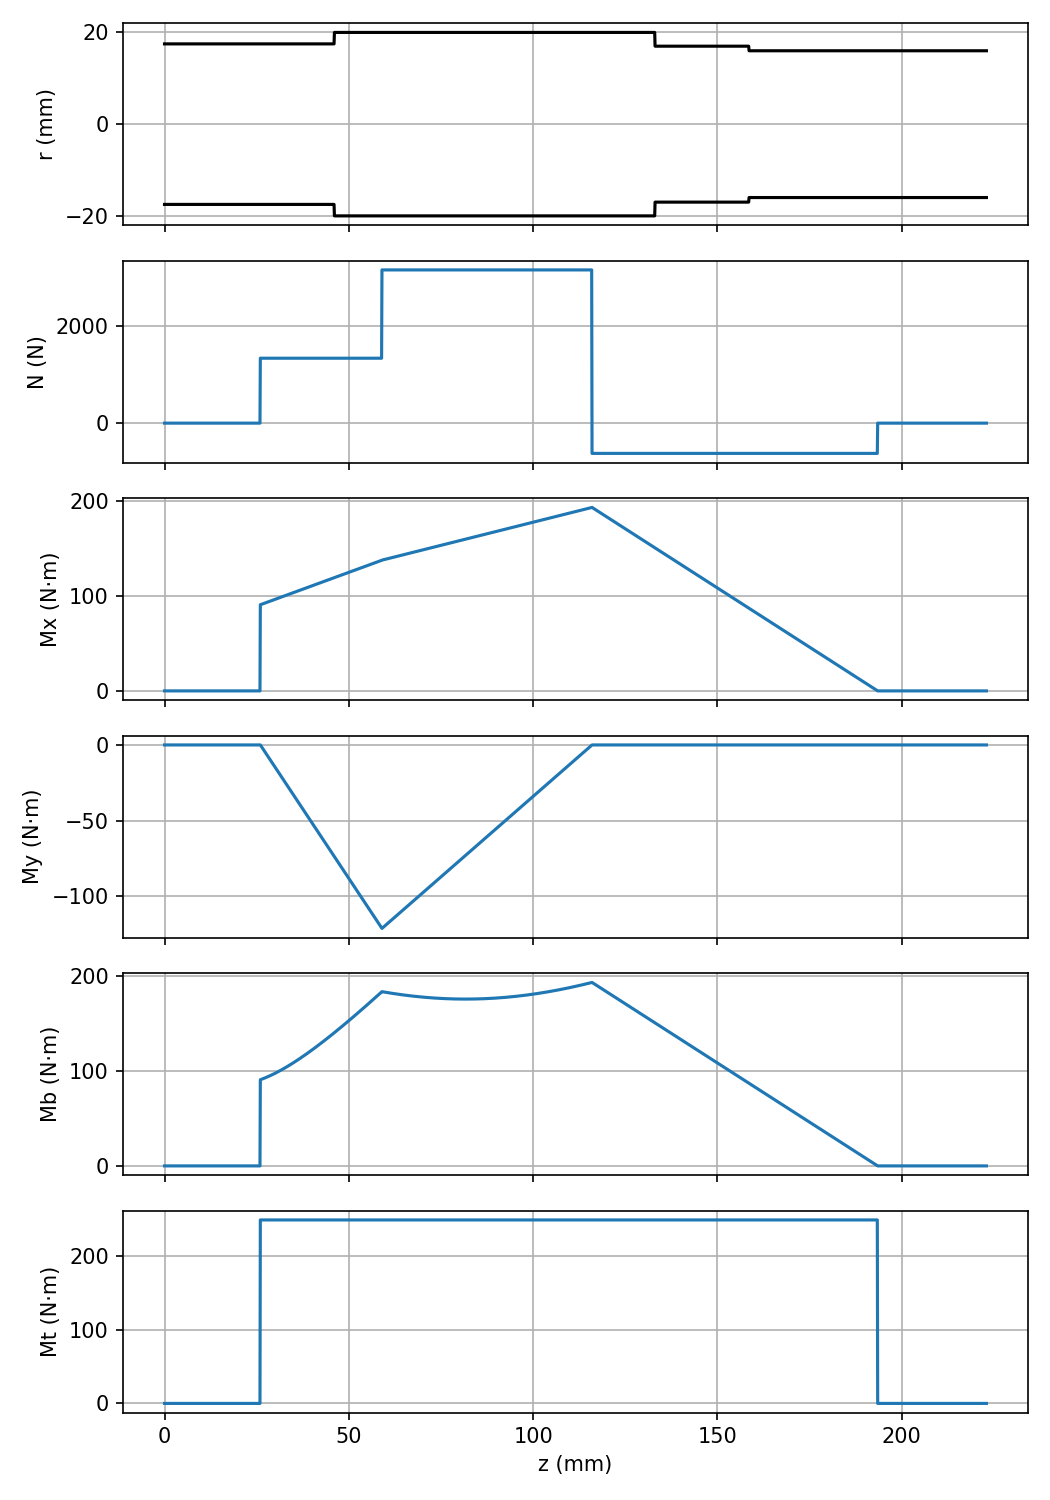
\includegraphics[width=0.8\textwidth,height=0.72\textheight,keepaspectratio]{../figures/internal_loads.png}
\caption{Shaft A2: diameter profile and internal loads along the shaft.}
\end{figure}
The total bending moment is largest at bearing D: $M_{B,\max}=193.35$\,N\,m at $z=116.0$\,mm. The torque $M_t=T_{A2}$ acts between the gear and the key L3.

\textbf{Stresses.} For the static check the keyseat sections use the nominal diameter minus the keyseat depth (5\,mm), and threads use their nominal diameter. The stresses are
\[\sigma_N=\frac{N}{A},\qquad \sigma_{M_B}=\frac{32M_B}{\pi d^3},\qquad \tau_{M_t}=\frac{16M_t}{\pi d^3},\]
\[\sigma_{tot}=|\sigma_N|+\sigma_{M_B},\qquad \sigma_{id}=\sqrt{\sigma_{tot}^2+3\tau^2},\qquad SF=\frac{\sigma_y}{\sigma_{id}}.\]
\begin{figure}[!htb]\centering
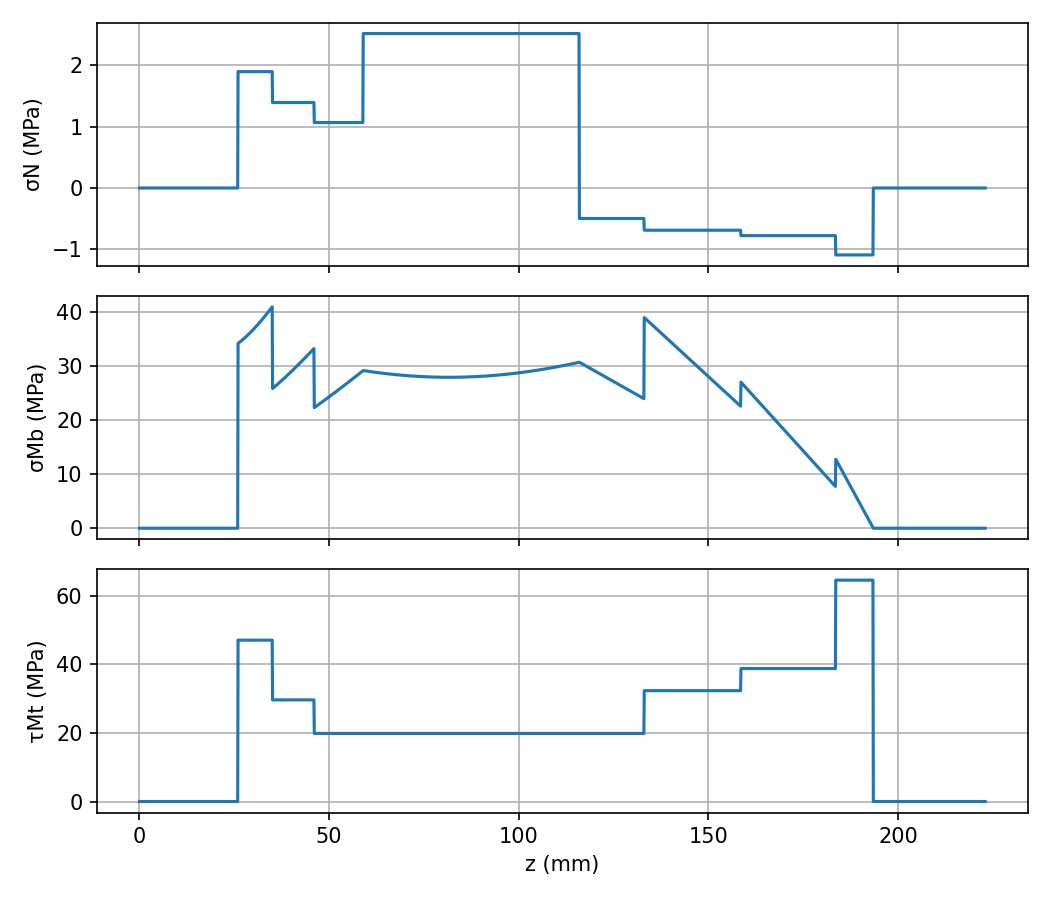
\includegraphics[width=0.85\textwidth]{../figures/stress_components.png}
\caption{Stress components along shaft A2 (static diameters).}
\end{figure}
\begin{figure}[!htb]\centering
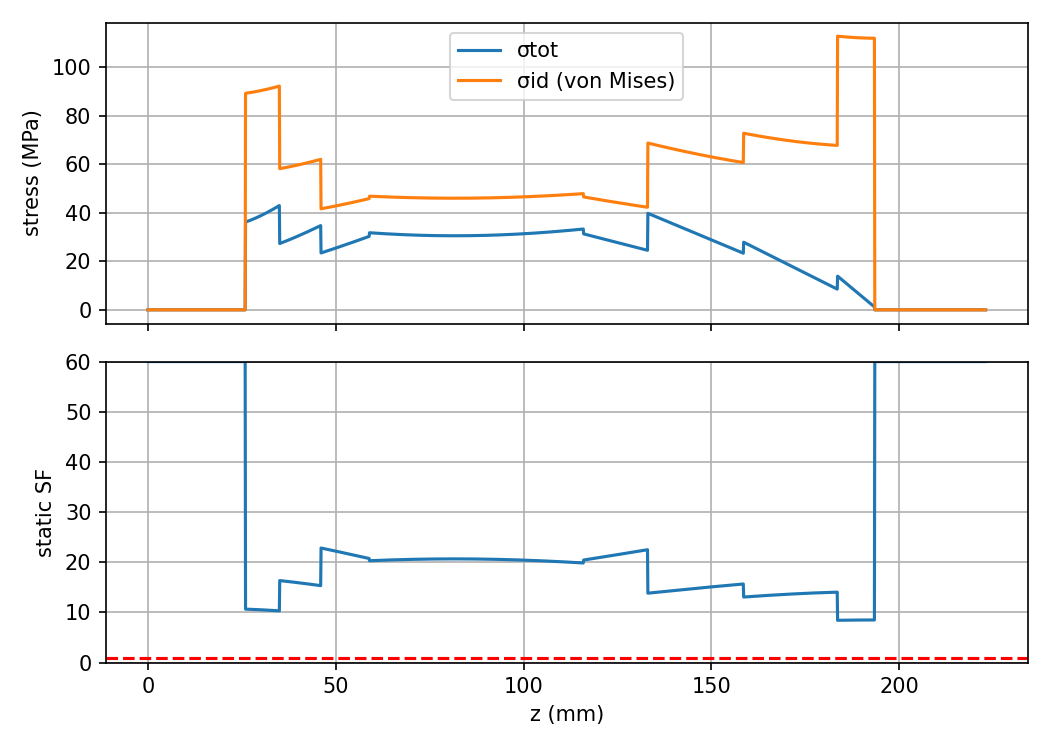
\includegraphics[width=0.85\textwidth]{../figures/stress_equivalent.png}
\caption{Total normal stress, von Mises equivalent stress and static safety factor along shaft A2.}
\end{figure}

\begin{table}[H]\centering\small
\caption{Static verification at the required sections (stresses in MPa).}
\setlength{\tabcolsep}{4.5pt}
\begin{tabular}{lrrrrrrrrr}\toprule
Section & $d$ (mm) & $N$ (N) & $M_B$ (N\,m) & $M_t$ (N\,m) & $\sigma_N$ & $\sigma_{M_B}$ & $\tau$ & $\sigma_{id}$ & $SF$\\\midrule
V1 (keyseat) & 30.00 & 1338.5 & 90.81 & 249.49 & 1.89 & 34.26 & 47.06 & 89.17 & \textbf{10.65}\\
V2 (shoulder) & 35.00 & 1338.5 & 140.15 & 249.49 & 1.39 & 33.29 & 29.64 & 61.95 & 15.33\\
V3 (shoulder) & 34.00 & \ensuremath{-}623.7 & 150.94 & 249.49 & \ensuremath{-}0.69 & 39.12 & 32.33 & 68.70 & 13.83\\\bottomrule
\end{tabular}\end{table}
The most critical required section is V1, with $SF_{s,\min}=10.65$. It is governed by torsion on the reduced diameter under keyseat L2. Outside the required sections, the keyseat for L3 has the lowest value along the whole shaft, $SF=8.43$ at $z\approx183.6$\,mm, which is still well above 1.

%=====================================================================================
\section{Shaft A2: fatigue verification}
%=====================================================================================
The shaft rotates, so bending is fully reversed ($\sigma_m^{M_B}=0$). The axial load and the torque are constant, so they contribute only mean components. Nominal stresses are computed on the full diameter, also at the keyseat (brief).

\textbf{Stress concentration.} At V1 the brief gives $K_f$ for the keyseat directly. At the shoulders V2 and V3 the fillet radius is $r=1$\,mm (details F and G of Fig.~4), so $r/d=0.029$. $K_t$ is read from the brief's charts and corrected with the notch sensitivity, $K_f=1+q(K_t-1)$ with $q=0.86$ ($r=1$\,mm, $\sigma_u=1.05$\,GPa).

\textbf{Fatigue limit.} The component fatigue limit is $\sigma_{D-1}^c=C_S\,C_F\,\sigma_{D-1}$, as in the course method. The 0.85 factor on the axial term in the Shigley equation already accounts for axial loading.

\textbf{Equivalent stresses (Shigley).}
\begin{align*}
\sigma_{a,eq}^P&=\sqrt{\Big(K_{f,B}\sigma_a^{B}+K_{f,N}\frac{\sigma_a^N}{0.85}\Big)^2+3\big(K_{f,T}\tau_a\big)^2},\\
\sigma_{m,eq}^P&=\sqrt{\big(K_{f,B}\sigma_m^{B}+K_{f,N}\sigma_m^N\big)^2+3\big(K_{f,T}\tau_m\big)^2}.
\end{align*}
\textbf{Safety factor.} All loads scale with the transmitted power, so the most appropriate definition is proportional loading ($\sigma_a/\sigma_m$ constant). It is measured to the Goodman line, $1/SF_f=\sigma_{a,eq}/\sigma_{D-1}^c+\sigma_{m,eq}/\sigma_u$, and checked against first-cycle yield.

\begin{table}[H]\centering\small
\caption{Fatigue verification of shaft A2 (stresses in MPa).}
\setlength{\tabcolsep}{4pt}
\begin{tabular}{lrrr}\toprule
 & V1 (keyseat) & V2 (shoulder) & V3 (shoulder)\\\midrule
$d$ / $D$ (mm) & 35 / -- & 35 / 40 & 34 / 40\\
$\sigma_a^{B}$ (nominal) & 21.57 & 33.29 & 39.12\\
$\sigma_m^{N}$ (nominal) & 1.39 & 1.39 & \ensuremath{-}0.69\\
$\tau_m$ (nominal) & 29.64 & 29.64 & 32.33\\
$K_{t,B}$ / $K_{t,N}$ / $K_{t,T}$ & -- & 2.22 / 2.43 / 1.59 & 2.24 / 2.57 / 1.72\\
$K_{f,B}$ / $K_{f,N}$ / $K_{f,T}$ & 1.600 / 1.600 / 2.000 & 2.053 / 2.233 / 1.504 & 2.070 / 2.353 / 1.622\\
$C_S$ / $C_F$ & 0.845 / 1 & 0.845 / 1 & 0.850 / 1\\
$\sigma_{D-1}^c$ & 439.40 & 439.40 & 442.00\\
$\sigma_{a,eq}^P$ / $\sigma_{m,eq}^P$ & 34.52 / 102.69 & 68.36 / 77.25 & 80.97 / 90.85\\
$SF_f$ (Goodman) / yield & 5.67 / 6.92 & 4.36 / 6.52 & \textbf{3.71} / 5.53\\\bottomrule
\end{tabular}\end{table}

\begin{figure}[!htb]\centering
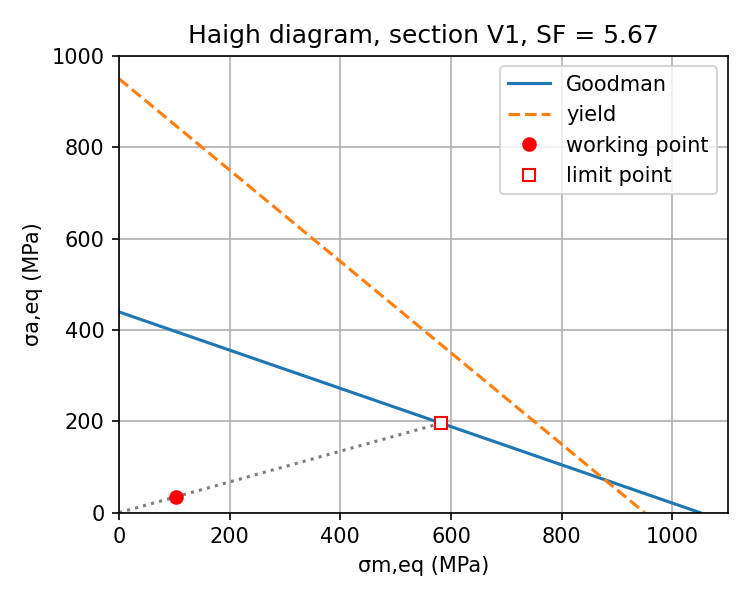
\includegraphics[width=0.49\textwidth]{../figures/haigh_V1.png}\hfill
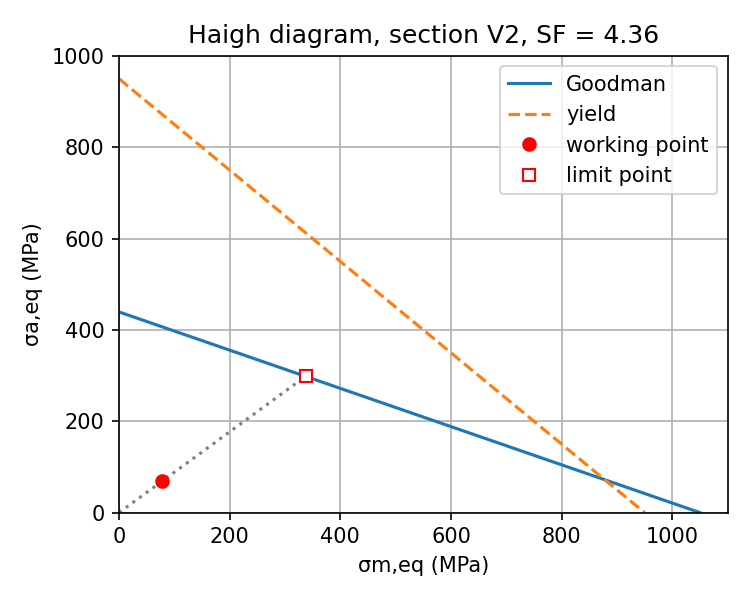
\includegraphics[width=0.49\textwidth]{../figures/haigh_V2.png}\\[4pt]
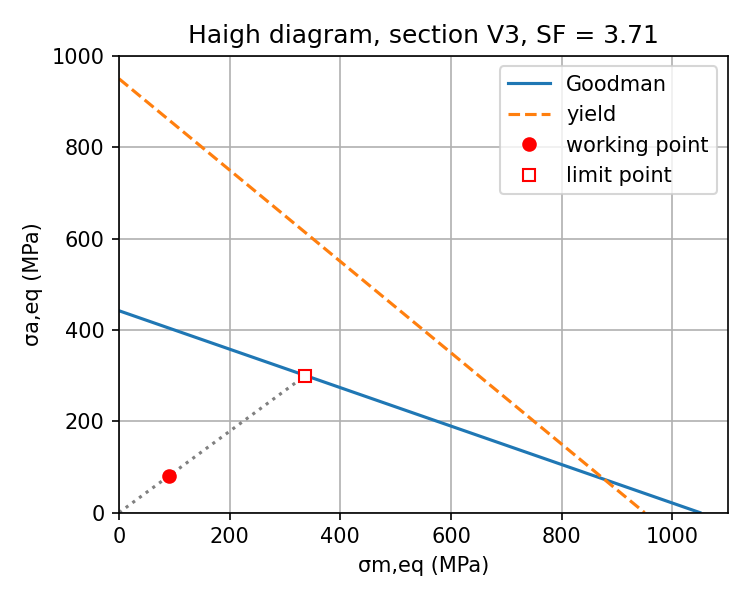
\includegraphics[width=0.49\textwidth]{../figures/haigh_V3.png}
\caption{Haigh diagrams for infinite life at V1, V2 and V3: working point and limit point along the proportional-loading line.}
\end{figure}
All three sections pass. The most critical section for fatigue is V3, with $SF_f=3.71$: it carries the highest bending stress on the smallest diameter, at a sharp 1\,mm fillet.

%=====================================================================================
\section{Gear verification (AGMA)}
%=====================================================================================
\[
\sigma_{\max,\mathrm{bending}}=F_tK_OK_BK_vK_HK_s\frac{1}{b\,m_tY_J},\qquad S_F=\frac{\sigma_{FP}}{\sigma_{\max,\mathrm{bending}}}\frac{Y_N}{Y_\theta Y_Z},
\]
\[
\sigma_{\max,\mathrm{pitting}}=Z_E\sqrt{F_tK_OK_vK_s\frac{K_H}{b\,d_P}\frac{Z_R}{Z_I}},\qquad S_H=\frac{\sigma_{HP}}{\sigma_{\max,\mathrm{pitting}}}\frac{Z_NZ_W}{Y_\theta Y_Z}.
\]
R3 runs on spindle P at 616.4\,rpm, not at the input speed. This sets its pitch-line velocity and therefore $K_v$.

\begin{table}[H]\centering\small
\caption{AGMA factors and results.}
\setlength{\tabcolsep}{4pt}
\begin{tabular}{p{4.9cm}rr}\toprule
 & R1 (mates R2) & R3 (mates R4)\\\midrule
Tangential load $F_t$ (N) & 957.16 & 3677.52\\
Pitch-line vel. $V_t$ (m/s, ft/min) & 6.27 / 1233.96 & 1.63 / 321.17\\
$K_O$ (uniform/uniform), $K_B$ & 1 / 1.00 (solid) & 1 / 1.00 ($m_B=1.271$)\\
$K_v$ ($Q_v=7$) & 1.3711 & 1.1946\\
$C_{pf}$ / $C_{pm}$ / $C_{ma}$ & 0.0399 / 1.10 (overhung) / 0.1455 & 0.0366 / 1.00 (brief) / 0.1455\\
$K_H$ & 1.1894 & 1.1821\\
$z'$, Lewis $Y$, $K_s$ & 21.69, 0.3301, 1.0345 & 22.90, 0.3337, 1.0348\\
$J'$ / $J''$ / $Y_J$ & 0.4940 / 0.9986 / 0.4933 & 0.4985 / 0.9837 / 0.4904\\
$Y_N$ / $Y_\theta$ / $Y_Z$ & 0.9768 / 1 / 1 & 0.9768 / 1 / 1\\
\textbf{$\sigma_{\max,\mathrm{bending}}$ (MPa) / $S_F$} & \textbf{41.01 / 7.62} & \textbf{137.31 / 3.20}\\\midrule
Load sharing ratio $m_N$ / $Z_I$ & 0.6505 / 0.2077 & 0.6573 / 0.1866\\
$Z_E$ ($\sqrt{\mathrm{MPa}}$) / $Z_R$ & 191 / 1 & 191 / 1\\
$Z_N$ / $HB_P/HB_G$ / $Z_W$ & 0.9484 / 0.60 / 1.0000 & 0.9484 / 1.67 / 1.0113\\
\textbf{$\sigma_{\max,\mathrm{pitting}}$ (MPa) / $S_H$} & \textbf{444.33 / 1.84} & \textbf{832.26 / 1.57}\\\bottomrule
\end{tabular}\end{table}
Both pinions pass in bending and in pitting. Pitting governs for both, and the lowest margin is R3 ($S_H=1.57$).

%=====================================================================================
\section{Bearings (SKF method)}
%=====================================================================================
\textbf{Equivalent loads.} SKF single-row equations for each bearing of the pair: $P=F_r$ if $F_a/F_r\le e$, otherwise $P=0.4F_r+YF_a$. The static load is $P_0=0.5F_r+Y_0F_a$, with $P_0=F_r$ if smaller.

\textbf{Minimum load.} SKF Explorer bearings need $F_{rm}=0.017\,C$, i.e.\ 0.398\,kN for 30203 and 1.289\,kN for 30208. Every bearing carries more than this.

\textbf{Life.} The SKF rating life at 95\,\% reliability is $L_{5m}=a_1a_{\mathrm{SKF}}(C/P)^{10/3}$ with $a_1=0.64$, and $L_{5mh}=10^6L_{5m}/(60n)$. The inputs are:
\begin{itemize}
\item oil viscosity at 60\,$^\circ$C: $\nu=40$\,mm$^2$/s;
\item rated viscosity $\nu_1(d_m,n)$, from the relation behind SKF diagram 14;
\item contamination factor $\eta_c=0.4$;
\item $a_{\mathrm{SKF}}$ from the radial-roller-bearing curves of SKF diagram 10, read on the Explorer axis.
\end{itemize}

\begin{table}[H]\centering\small
\caption{Bearing loads, static check and rating life.}
\begin{tabular}{lrrrr}\toprule
 & A (30203) & B (30203) & C (30208) & D (30208)\\\midrule
$n$ (rpm) & 2500.0 & 2500.0 & 229.7 & 229.7\\
$F_r$ / $F_a$ (kN) & 1.033 / 0.952 & 2.053 / 0.604 & 5.824 / 1.820 & 4.071 / 3.782\\
$F_a/F_r$ ($e$) & 0.922 (0.35) & 0.294 (0.35) & 0.312 (0.37) & 0.929 (0.37)\\
$P$ (kN) & 2.032 & 2.053 & 5.824 & 7.680\\
$P_0$ (kN) / $s_0=C_0/P_0$ & 1.373 / 13.54 & 2.053 / 9.06 & 5.824 / 11.68 & 5.439 / 12.50\\
$\nu_1$ (mm$^2$/s) / $\kappa$ & 16.86 / 2.37 & 16.86 / 2.37 & 63.75 / 0.63 & 63.75 / 0.63\\
$\eta_cP_u/P$ / $a_{\mathrm{SKF}}$ & 0.360 / 3.57 & 0.357 / 3.51 & 0.525 / 0.85 & 0.398 / 0.67\\
$L_{10}$ / $L_{5m}$ (Mrev) & 3450 / 7892 & 3334 / 7492 & 5186 / 2837 & 2063 / 879\\
\textbf{$L_{5mh}$ (h)} & \textbf{52\,614} & \textbf{49\,948} & \textbf{205\,893} & \textbf{63\,792}\\\bottomrule
\end{tabular}\end{table}
All bearings exceed the minimum load and have static safety factors above 9. The shortest life is bearing B, about $5\times10^4$\,h. The output bearings C and D run in mixed lubrication ($\kappa<1$), which lowers $a_{\mathrm{SKF}}$ below 1, but their low speed keeps the lives long.

%=====================================================================================
\section{Submission tables}
%=====================================================================================
\begin{table}[H]\centering\small
\begin{minipage}[t]{0.48\textwidth}\centering
\caption*{Shaft analysis (m.c.s.\ for fatigue: V3)}
\begin{tabular}{lrl}
\toprule
Quantity & Value & Unit \\
\midrule
$R_{x,C}$ & \ensuremath{-}5806.6 & N \\
$R_{y,C}$ & \ensuremath{-}450.0 & N \\
$R_{x,D}$ & 2129.1 & N \\
$R_{y,D}$ & \ensuremath{-}3469.3 & N \\
$R_{z,C}$ & \ensuremath{-}1820.0 & N \\
$R_{z,D}$ & 3782.2 & N \\
\midrule
$M_x$ (V1) & 90.81 & N\,m \\
$M_x$ (V2) & 119.29 & N\,m \\
$M_x$ (V3) & 150.94 & N\,m \\
$M_y$ (V1) & 0.00 & N\,m \\
$M_y$ (V2) & \ensuremath{-}73.55 & N\,m \\
$M_y$ (V3) & 0.00 & N\,m \\
$N$ (V1) & 1338.5 & N \\
$N$ (V2) & 1338.5 & N \\
$N$ (V3) & \ensuremath{-}623.7 & N \\
$M_{B,\mathrm{tot,max}}$ & 193.35 & N\,m \\
$M_{t,\max}$ & 249.49 & N\,m \\
$SF$ (static) & 10.65 & -- \\
\midrule
$\sigma_{a,b}^{\mathrm{nom}}$ (V3) & 39.12 & MPa \\
$\sigma_{m,b}^{\mathrm{nom}}$ (V3) & 0.00 & MPa \\
$\sigma_{a,N}^{\mathrm{nom}}$ (V3) & 0.00 & MPa \\
$\sigma_{m,N}^{\mathrm{nom}}$ (V3) & \ensuremath{-}0.69 & MPa \\
$\tau_{a,t}^{\mathrm{nom}}$ (V3) & 0.00 & MPa \\
$\tau_{m,t}^{\mathrm{nom}}$ (V3) & 32.33 & MPa \\
$K_{f,b}$ & 2.070 & -- \\
$\sigma_{a,b}^{\mathrm{eff}}$ (V3) & 80.97 & MPa \\
$\sigma_{m,b}^{\mathrm{eff}}$ (V3) & 0.00 & MPa \\
$K_{f,N}$ & 2.353 & -- \\
$\sigma_{a,N}^{\mathrm{eff}}$ (V3) & 0.00 & MPa \\
$\sigma_{m,N}^{\mathrm{eff}}$ (V3) & \ensuremath{-}1.62 & MPa \\
$K_{f,T}$ & 1.622 & -- \\
$\tau_{a,t}^{\mathrm{eff}}$ (V3) & 0.00 & MPa \\
$\tau_{m,t}^{\mathrm{eff}}$ (V3) & 52.44 & MPa \\
$\sigma_{a,\mathrm{eq}}^{P}$ (V3) & 80.97 & MPa \\
$\sigma_{m,\mathrm{eq}}^{P}$ (V3) & 90.85 & MPa \\
$SF_f$ (fatigue) & 3.71 & -- \\
\bottomrule
\end{tabular}
\end{minipage}\hfill
\begin{minipage}[t]{0.48\textwidth}\centering
\caption*{Gears -- AGMA verification}
\begin{tabular}{lrl}
\toprule
Quantity & Value & Unit \\
\midrule
\multicolumn{3}{l}{\textbf{Gear R1 -- bending}} \\
$F_t/(b\,m_t\,Y_J)$ & 24.31 & MPa \\
$\sigma_{\max,\mathrm{bending}}$ & 41.01 & MPa \\
$S_F$ & 7.62 & -- \\
\multicolumn{3}{l}{\textbf{Gear R1 -- pitting}} \\
$Z_E\sqrt{F_t/(b\,d_P)\cdot 1/Z_I}$ & 342.10 & MPa \\
$\sigma_{\max,\mathrm{pitting}}$ & 444.33 & MPa \\
$S_H$ & 1.84 & -- \\
\multicolumn{3}{l}{\textbf{Gear R3 -- bending}} \\
$F_t/(b\,m_t\,Y_J)$ & 93.96 & MPa \\
$\sigma_{\max,\mathrm{bending}}$ & 137.31 & MPa \\
$S_F$ & 3.20 & -- \\
\multicolumn{3}{l}{\textbf{Gear R3 -- pitting}} \\
$Z_E\sqrt{F_t/(b\,d_P)\cdot 1/Z_I}$ & 688.47 & MPa \\
$\sigma_{\max,\mathrm{pitting}}$ & 832.26 & MPa \\
$S_H$ & 1.57 & -- \\
\bottomrule
\end{tabular}\\[10pt]
\caption*{Bearings -- loads}
\begin{tabular}{lrl}
\toprule
Quantity & Value & Unit \\
\midrule
$F_{r,A}$ & 1.033 & kN \\
$F_{a,A}$ & 0.952 & kN \\
$P_{A}$ & 2.032 & kN \\
$F_{r,B}$ & 2.053 & kN \\
$F_{a,B}$ & 0.604 & kN \\
$P_{B}$ & 2.053 & kN \\
$F_{r,C}$ & 5.824 & kN \\
$F_{a,C}$ & 1.820 & kN \\
$P_{C}$ & 5.824 & kN \\
$F_{r,D}$ & 4.071 & kN \\
$F_{a,D}$ & 3.782 & kN \\
$P_{D}$ & 7.680 & kN \\
\bottomrule
\end{tabular}\\[10pt]
\caption*{Bearings -- corrected rating life}
\begin{tabular}{lrl}
\toprule
Quantity & Value & Unit \\
\midrule
$\kappa_A$ & 2.37 & -- \\
$\kappa_B$ & 2.37 & -- \\
$\kappa_C$ & 0.63 & -- \\
$\kappa_D$ & 0.63 & -- \\
$a_{\mathrm{SKF},A}$ & 3.57 & -- \\
$a_{\mathrm{SKF},B}$ & 3.51 & -- \\
$a_{\mathrm{SKF},C}$ & 0.85 & -- \\
$a_{\mathrm{SKF},D}$ & 0.67 & -- \\
$L_{5mh,A}$ & 52\,614 & h \\
$L_{5mh,B}$ & 49\,948 & h \\
$L_{5mh,C}$ & 205\,893 & h \\
$L_{5mh,D}$ & 63\,792 & h \\
\bottomrule
\end{tabular}
\end{minipage}
\end{table}

%=====================================================================================
\appendix
\section{Chart readings and assumptions}
%=====================================================================================
\begin{itemize}
\item \textbf{Helix hands:} read from the slant marks in Fig.~2 of the brief using the convention on slide~21 of the course presentation. R1 and R4 are right-handed; R2 and R3 are left-handed.
\item \textbf{Bearing pressure centres:} at distance $a$ from the inner face of each bearing (outboard shift for back-to-back mounting).
\item \textbf{$K_t$ at $r/d=0.029$ (brief, p.~10):}
  \begin{itemize}
  \item bending: 2.20 ($D/d=1.1$), 2.43 ($D/d=1.5$);
  \item torsion: 1.41 ($D/d=1.1$), 1.82 ($D/d=1.2$);
  \item axial: 2.05 ($D/d=1.05$), 2.67 ($D/d=1.2$, extrapolated because that curve starts at $r/d\approx0.04$).
  \end{itemize}
  Values in between are interpolated linearly in $D/d$.
\item \textbf{Keyseat factor at V1:} the brief gives bending 1.6 and torsion 2.0. The bending value is also used for the (very small) axial mean stress.
\item \textbf{Other fatigue factors:} notch sensitivity $q=0.86$; size factor $C_S=0.845$ (d = 35\,mm) and 0.85 (34\,mm); surface factor $C_F=1$ (Ra $\le0.8\,\mu$m).
\item \textbf{AGMA chart values:}
  \begin{itemize}
  \item $K_v$ from the analytic form of the $Q_v=7$ curve;
  \item $C_{pf}$ and $C_{ma}$ (commercial enclosed units) from the AGMA equations behind the charts;
  \item $C_{pm}=1.1$ for R1, because it overhangs bearing B (cantilever); $C_{pm}=1$ for R3 (brief);
  \item $J'$ at $\psi=20^\circ$ from the actual tooth numbers (0.503 at 20 teeth, 0.548 at 30), since the chart is already plotted against helix angle;
  \item $J''$ from the mating gear's tooth number (0.983 at 50 teeth, 1.000 at 75);
  \item Lewis $Y$ at the virtual tooth number (brief).
  \end{itemize}
\item \textbf{SKF values:}
  \begin{itemize}
  \item viscosity: 40\,mm$^2$/s for VG\,100 at 60\,$^\circ$C (diagram 13);
  \item $\eta_c=0.4$, the middle of the 0.5--0.3 range for slight contamination;
  \item $a_{\mathrm{SKF}}$ from the ISO\,281 roller-bearing relation that the curves of diagram 10 follow, read on the Explorer axis, which sits a factor 1.39 to the right of the standard axis.
  \end{itemize}
\end{itemize}

\section{Changes from the January 2025 submission}
This revision recalculates the whole project from the brief. The main corrections are:
\begin{itemize}
\item \textbf{Axial gear forces.} The original used $\tan(20)$ evaluated in radians, which gave 2142 and 8229\,N instead of 348.4 and 1338.5\,N. It also omitted the $1/\cos\psi$ factor in the radial forces.
\item \textbf{Output torque and end-user force.} The original computed the end-user force from the intermediate torque, 92.96\,N\,m instead of 249.49\,N\,m, which gave 930\,N instead of 2494.9\,N.
\item \textbf{Axial-force couple.} The original applied the couple $F_a r$ in both planes, with the Ft--Fr resultant used as the axial force. This inflated $M_{B,\max}$ to 775\,N\,m, against 193.35\,N\,m here.
\item \textbf{Fatigue.} The original evaluated fatigue only at V3; it is now evaluated at all three sections with Haigh diagrams. The torsional stress at V3 now uses the correct diameter.
\item \textbf{AGMA.}
  \begin{itemize}
  \item $1/(b\,m_tY_J)$ was applied as a product, with $m_t=6.86$\,mm.
  \item R1 was evaluated with the R3--R4 mesh force.
  \item The speed of R3 was taken as the input speed.
  \item $Q_v$ was quoted as 8, $C_{pm}$ was swapped between R1 and R3, and $Z_I\approx0.85$ was used instead of about 0.2.
  \end{itemize}
\item \textbf{Bearings.} The (10/3) exponent was missing for bearing B. The original used $P_0=F_r+Y_0F_a$, and converted lives to hours without $10^6/(60n)$, which gave lives of 22--1065\,h.
\end{itemize}
The revised results show that every component passes. The governing margins are fatigue of A2 at V3 ($SF_f=3.71$) and pitting of R3 ($S_H=1.57$).
\end{document}